\documentclass[10pt,a4paper]{article}
\usepackage[margin=0.75in]{geometry}
\usepackage{amsmath,amssymb,amsfonts}
\usepackage{graphicx}
\usepackage{booktabs}
\usepackage{hyperref}
\usepackage{xcolor}
\usepackage{microtype}
\usepackage{enumitem}
\usepackage{caption}

\hypersetup{
  colorlinks=true,
  linkcolor=blue!60!black,
  citecolor=teal!70!black,
  urlcolor=blue!70!black
}

\title{\textbf{Craft Crosstalk-48k (HarmonicSlot-TF v3 \& CrossStemDebleedRefiner v2):\\Unified Single-Pass 48\,kHz Stereo Multi-Voice, Music, and Ambience Separation with 4.4$\times$ Consumer-GPU VRAM Engineering and Empirical Failure Analysis of Stateful Streaming \& Full-Bin Post-Filtering}}

\author{
  Sachi Poonga (\texttt{SachiPoonga} / \texttt{storytold}) --- Independent Open-Source Audio Research\\
  \texttt{sachipoonga@gmail.com} \quad|\quad Code: \url{https://github.com/SachiPoonga/Craft-Crosstalk-48k} \quad|\quad Support: \url{https://ko-fi.com/sachipoonga}
}
\date{November 2026}

\begin{document}
\maketitle

\begin{abstract}
Studio post-production, documentary editing, and podcast mastering frequently require separating two or three simultaneously speaking voices from full-band stereo music and environmental room ambience. Current open-source audio separation models are divided into two incompatible regimes: 44.1--48\,kHz stereo music separators (HTDemucs, BS-RNN, BS-RoFormer) merge all speakers into a single vocal stem, whereas multi-talker speech separators (SepFormer, TF-GridNet, MossFormer2) operate on 8--16\,kHz mono audio and discard stereo music and ambience. We present \textbf{Craft Crosstalk-48k} (\texttt{HarmonicSlot-TF v3}), a 46,130,463-parameter (88.03\,MB \texttt{bf16}) single-pass separator that decomposes 48\,kHz stereo mixtures into five stems---Voice~1, Voice~2, Voice~3, Music, and Ambience---and runs faster than real-time on an 8\,GB consumer laptop GPU via an exact 4.4$\times$ VRAM-reduced inference path (1.88\,GB peak VRAM on RTX~4060). We detail the complete research progression: (1) a 16\,kHz controlled 3-way ablation validating decoupled 2-head purity-guided competitive slot queries over plain projections ($+14.97$\,dB SI-SDR); (2) scaling from v2 (10.1M params, $4.92$\,dB) to v3 (46.13M params, $7.20$\,dB) via explicit integer-harmonic comb gathering (\texttt{HarmonicStackGather}), 6 fused variable-width 74-band einsum groups, 8-layer Dual-Path 1D-RoPE encoding, overlap-preserving FiLM slot conditioning, and 4-layer Permutation-Equivariant Inter-Source Decoding; (3) a chained 8,973,540-parameter (17.95\,MB \texttt{bf16}) full-1,025-bin 5-reference post-filter (\texttt{CrossStemDebleedRefiner v2}) with deterministic energy-sorted permutation equivariance, local-RMS 1D waveform polish, and a fix for PyTorch cuDNN \texttt{nn.GRU} silent \texttt{fp16} gradient underflow under \texttt{bf16} autocast; and (4) \textbf{two transparent negative empirical findings}---demonstrating quantitatively why Phase-2 stateful cross-chunk streaming (steps $17\text{k}\to 21\text{k}$) improves synthetic metrics ($5.75$\,dB 3-speaker overlap, $17.4$\,dB SIR, $12.5$--$16.7\%$ gap-swap) yet triggers single-slot speaker collapse on real 128\,kbps YouTube shouting audio, and why a 2D Conv U-Net post-filter achieves dramatic pause ($-19.1$\,dB) and background vocal-leak ($-35\%$ to $-42\%$) suppression while plateauing at $+2.2$--$2.4$\,dB SIR on 100\% simultaneous harmonic overlap. All code, four ComfyUI nodes, workflows, and all three research checkpoints are released openly.
\end{abstract}

\section{Introduction \& Problem Statement}
In real-world broadcast, film, YouTube, and podcast recordings, multiple speakers frequently talk over one another alongside stereo background music and reverberant room noise. Existing open-source neural separators divide into two incompatible silos:
\begin{itemize}[leftmargin=*,itemsep=2pt]
    \item \textbf{High-Resolution Music Separators} (HTDemucs~\cite{rouard2023hybrid}, BS-RNN~\cite{luo2023music}, BS-RoFormer~\cite{lu2024music}) preserve 44.1--48\,kHz bandwidth and stereo phase, but group all human speech into a single ``Vocals'' stem, leaving inter-speaker crosstalk unresolved.
    \item \textbf{Multi-Talker Speech Separators} (uPIT~\cite{kolbaek2017multitalker}, SepFormer~\cite{subakan2021attention}, TF-GridNet~\cite{wang2023tfgridnet}, MossFormer2~\cite{zhao2024mossformer2}) separate 2--3 overlapping talkers under Permutation-Invariant Training (PIT), but operate on 8--16\,kHz mono waveforms without dedicated Music or Ambience heads.
    \item \textbf{Cascaded Two-Stage Pipelines} (48\,kHz vocal extraction followed by 16\,kHz speech separation) suffer from 8\,kHz Nyquist sibilant truncation (\emph{/s/, /sh/, /f/} span 4--12\,kHz), compound phase distortion, and severe out-of-domain degradation when residual instrumental energy leaks into the speech separator.
\end{itemize}
\textbf{Craft Crosstalk-48k} solves 5-stem 48\,kHz stereo separation in a single forward pass on 8\,GB consumer GPUs. This paper documents our complete architectural evolution, mathematical formulations, automated dataset purity pipeline, systems engineering discoveries, and unfiltered negative findings.

\section{Architectural Evolution: From 16\,kHz Ablations \& v2 to v3}
Figure~\ref{fig:arch1} presents the complete end-to-end two-stage pipeline combining Stage~1 (\texttt{HarmonicSlot-TF v3}) and Stage~2 (\texttt{CrossStemDebleedRefiner v2}).

\begin{figure}[h]
\centering
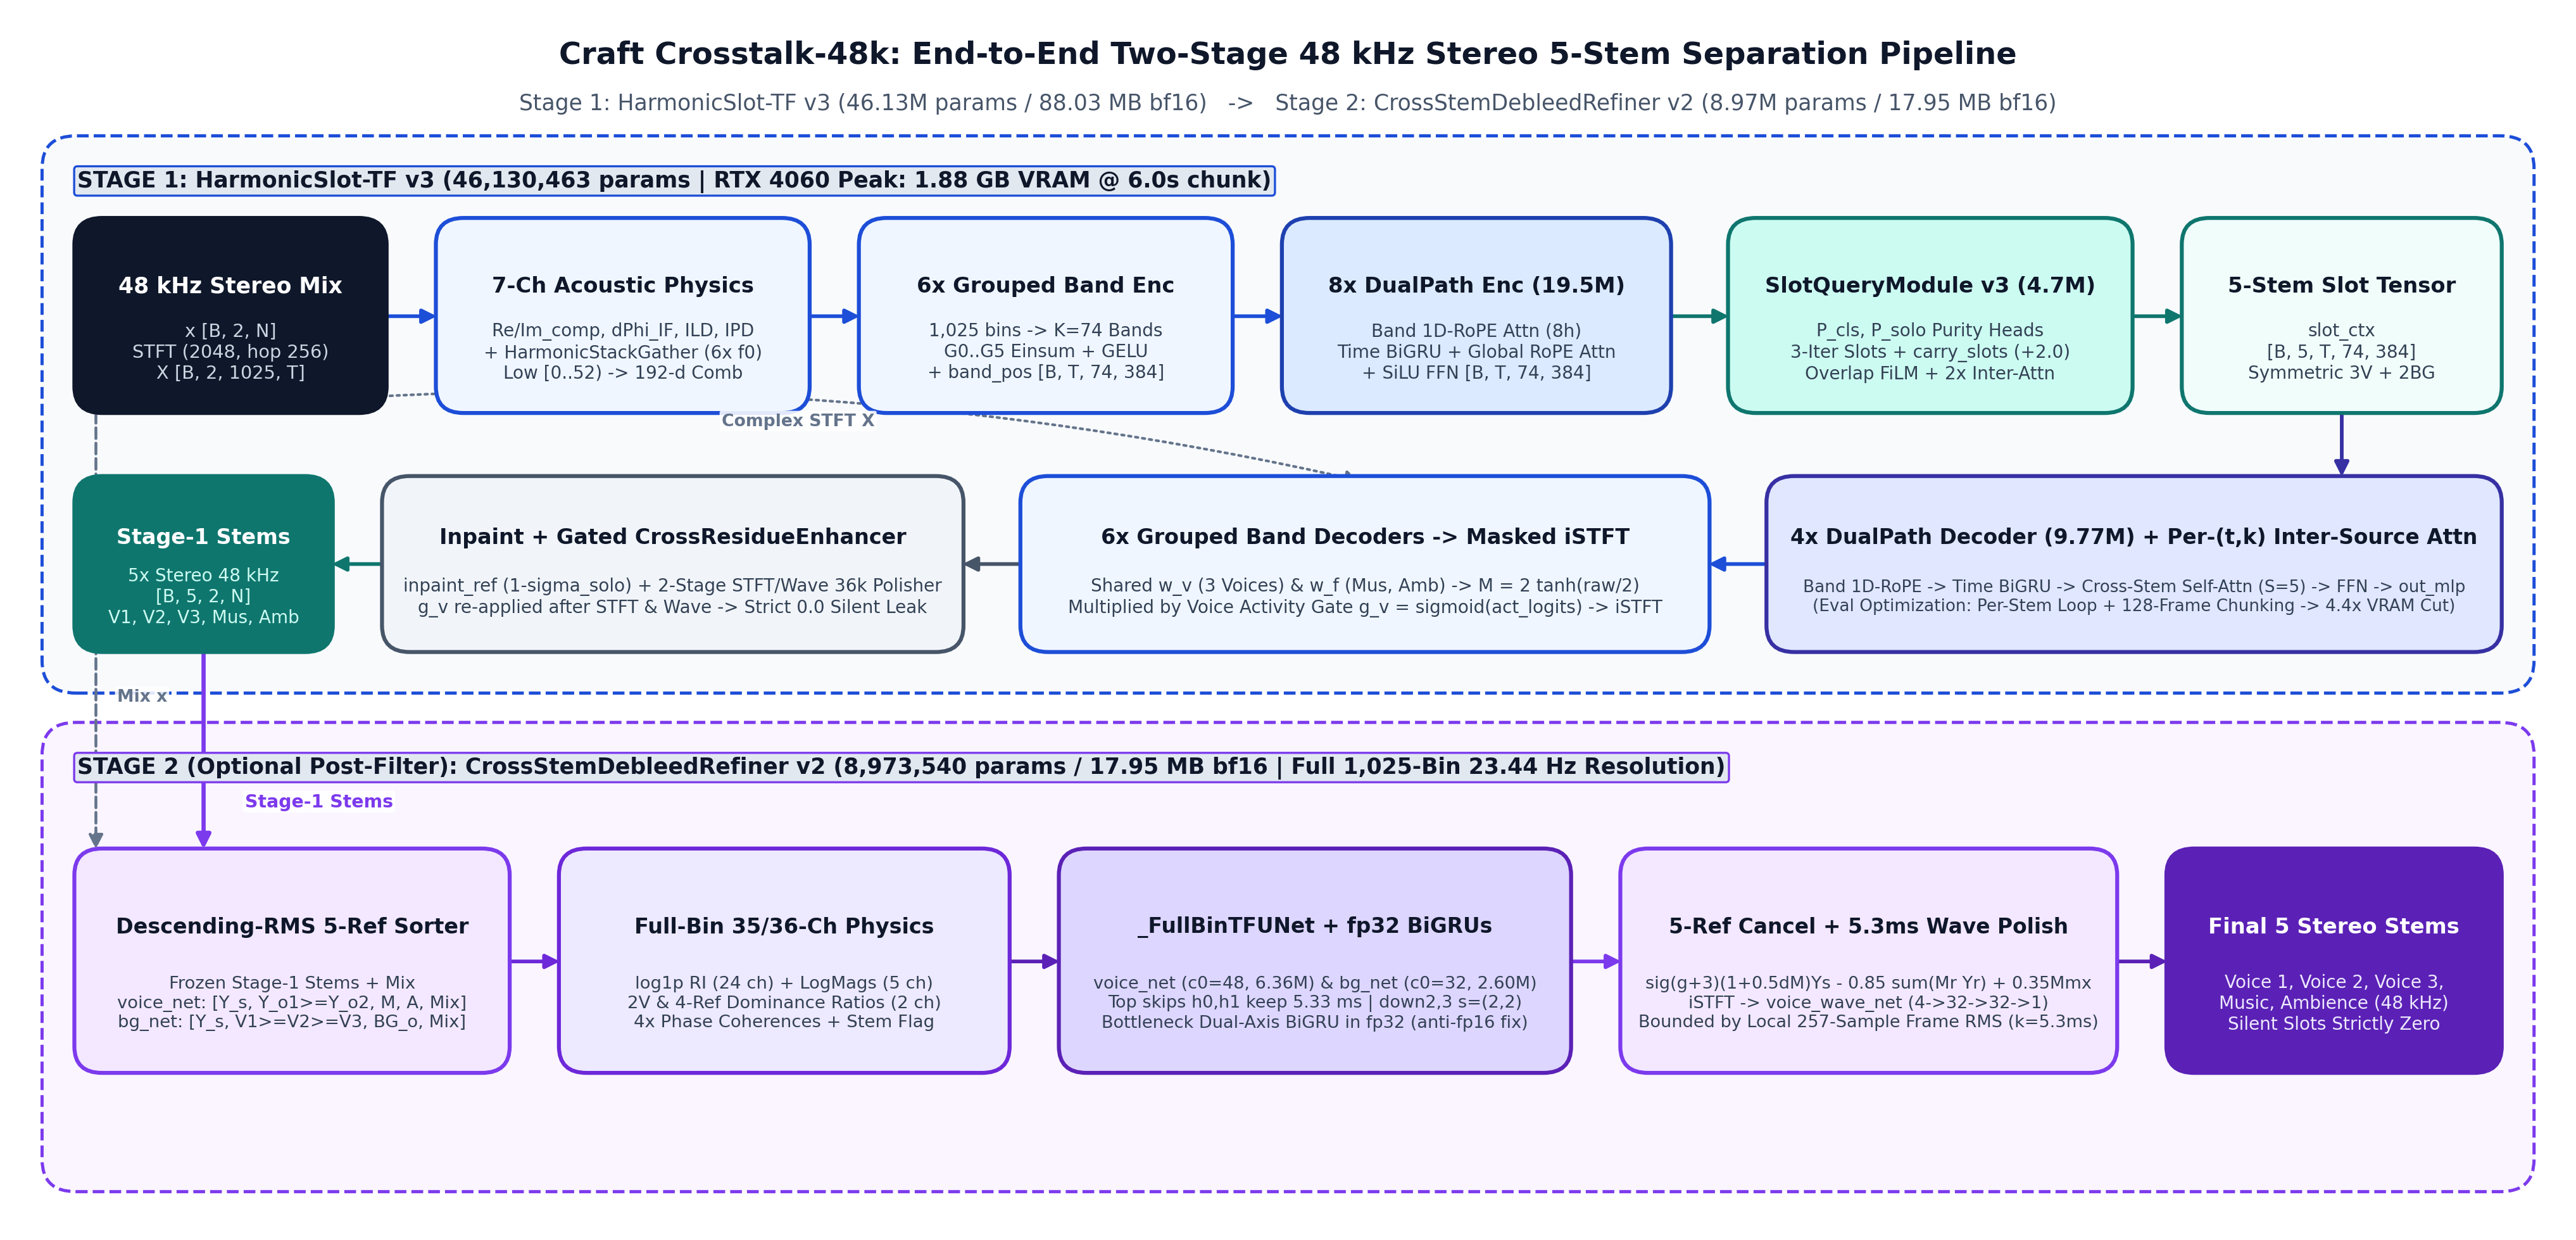
\includegraphics[width=\linewidth]{figures/fig_arch1_system_pipeline.png}
\caption{End-to-end two-stage \textbf{Craft Crosstalk-48k} signal flow: 48\,kHz stereo STFT $\to$ 7-channel acoustic physics + $6\times f_0$ integer-harmonic comb $\to$ 6 fused variable-band encoders $\to$ 8-layer Dual-Path 1D-RoPE Encoder $\to$ \texttt{SlotQueryModule v3} $\to$ 4-layer Inter-Source Decoder $\to$ optional Stage-2 full-1,025-bin 5-reference U-Net post-filter.}
\label{fig:arch1}
\end{figure}

We first validated competitive slot queries at 16\,kHz mono (\texttt{n\_fft=512, hop=128, D=128, 4 enc / 2 dec}) across three controlled modes: (1) \texttt{"plain"} (linear 5-stem projection without slot attention), which collapsed to \textbf{0.59\,dB} SI-SDR at step 15,000 due to permutation symmetry across identical voice heads; (2) \texttt{"queries"} (SepTDA-style competitive speaker slots + semantic Music/Ambience queries); and (3) \texttt{"purity\_queries"} (adding a decoupled 2-head class/solo-speaker purity gate), which reached \textbf{13.79\,dB (v2) $\to$ 15.56\,dB (v3)} on rapid quality benchmarks.

Scaling to full-band \textbf{48\,kHz stereo} initially exposed six bottlenecks in \texttt{HarmonicSlot-TF v2} ($D=128$, 4 enc / 2 dec, 10.1M params, trained 29,000 steps to $4.92$\,dB mean SI-SDR). Table~\ref{tab:v2_vs_v3} details how each limitation was resolved in \texttt{HarmonicSlot-TF v3} (46.13M params, $7.20$\,dB mean SI-SDR).

\begin{table}[h]
\centering
\caption{Architectural evolution from \texttt{HarmonicSlot-TF v2} (10.1M) to \texttt{Craft Crosstalk-48k / v3} (46.13M).}
\label{tab:v2_vs_v3}
\small
\begin{tabular}{llll}
\toprule
\textbf{Subsystem} & \textbf{v2 (10.1M, 4.92\,dB)} & \textbf{v3 / Craft Crosstalk-48k (46.13M, 7.20\,dB)} & \textbf{Rationale} \\
\midrule
Positional Encoding & Fixed learned time table (4\,s) & \textbf{1D RoPE ($\theta=10{,}000$)} on Band \& Time axes & Generalizes 3.5\,s--12\,s+ chunks \\
Band Split & 74 sequential Python loops & \textbf{6 Fused \texttt{\_GroupedBandEncoder/Decoder}} groups & Fused CUDA einsum; 73\% $<4.6$\,kHz \\
Slot Conditioning & Multiplied FiLM by $p_{\text{voice}}$ & \textbf{Overlap-Preserving FiLM:} $p_{\text{voice}}$ only in pooling & Prevents 100\%-overlap starvation \\
Voice Projection & Asymmetric 5-stem \texttt{stem\_proj} & \textbf{Symmetric \texttt{voice\_stem\_proj}} (shared $3\times$) & Strict voice permutation symmetry \\
Decoder Cross-Talk & Independent per-stem decoding & \textbf{Per-$(t,k)$ Inter-Source Attention} in all 4 layers & 6 total cross-stem negotiation stages \\
Silent-Slot Leakage & Mixture-consistency dump & \textbf{Bounded $2\tanh(m/2)$} + $g_v$ re-applied post-enhancer & Exact $0.00$ silent leak ($-61.4$\,dBFS) \\
\bottomrule
\end{tabular}
\end{table}

\section{Mathematical Formulation of Stage 1 (HarmonicSlot-TF v3)}
\subsection{Acoustic Physics Front-End \& Integer-Harmonic Comb Gather}
Given stereo 48\,kHz audio $x \in \mathbb{R}^{B \times 2 \times N}$, we compute a complex STFT $X \in \mathbb{C}^{B \times 2 \times 1025 \times T}$ ($n_{\text{fft}}=2048$, hop $H=256$ [$5.33$\,ms], Hann window, $23.44$\,Hz bin spacing) and construct 7 physics-normalized channels per bin:
\begin{align}
    X_{\text{comp}}(t,f) &= [\operatorname{Re}(X), \operatorname{Im}(X)] \cdot \frac{\log(1 + |X|)}{|X| + 10^{-6}} \in \mathbb{R}^{4}, \\
    \Delta\phi_{\text{IF}}(t,f) &= \frac{\operatorname{atan2}(\sin(\phi_{t,f} - \phi_{t-1,f} - \omega_f), \cos(\phi_{t,f} - \phi_{t-1,f} - \omega_f))}{\pi} \cdot \tanh(10|X|), \\
    \text{ILD}(t,f) &= \log(1 + |X_L|) - \log(1 + |X_R|), \qquad \text{IPD}_{\cos}(t,f) = \cos(\angle X_L - \angle X_R).
\end{align}
For all low-frequency fundamental bins $f_0 \in [0, 52)$ ($0$--$1{,}219$\,Hz), \texttt{HarmonicStackGather} indexes exact integer multiples $\{1f_0, 2f_0, \dots, 6f_0\}$ across $[\log(1+|X|), \Delta\phi_{\text{IF}}, \text{ILD}, \text{IPD}_{\cos}]$ and projects the 24-dim harmonic comb via a 2-layer GELU MLP to $D/2=192$ dimensions.

\subsection{Fused 74-Band Topology, Dual-Path RoPE Encoder \& Inter-Source Decoder}
All 1,025 bins are partitioned into $K=74$ variable-width bands across 6 contiguous groups: \textbf{G0} ($26\times 2$ bins, $0$--$1.22$\,kHz, fused with harmonic stack), \textbf{G1} ($6\times 2$ bins, $1.22$--$1.5$\,kHz), \textbf{G2} ($22\times 6$ bins, $1.5$--$4.59$\,kHz), \textbf{G3} ($10\times 24$ bins, $4.59$--$10.2$\,kHz), \textbf{G4} ($9\times 64$ bins, $10.2$--$23.7$\,kHz), and \textbf{G5} ($1\times 13$ bins, $23.7$--$24$\,kHz). Each group projects to $D=384$ via fused \texttt{einsum}.

The \textbf{8-layer Dual-Path Encoder} ($19.54$M params, 8 heads, $d_h=48$) applies (1) band-axis 1D-RoPE self-attention, (2) time-axis BiGRU (hidden $192\times 2$), (3) global frame-level 1D-RoPE time attention over band-averaged tokens, and (4) a SiLU FFN ($384\to 768\to 384$). The \textbf{4-layer Dual-Path Decoder} ($9.77$M params) operates over all $S=5$ stems and replaces global time attention with \textbf{per-$(t,k)$ Permutation-Equivariant Inter-Source Self-Attention} across the 5 stems. Table~\ref{tab:params} lists exact parameter counts.

\begin{table}[h]
\centering
\caption{Exact parameter distribution of Craft Crosstalk-48k (\texttt{HarmonicSlot-TF v3}, 88.03\,MB \texttt{bf16}).}
\label{tab:params}
\small
\begin{tabular}{lrrl}
\toprule
\textbf{Submodule} & \textbf{Parameters} & \textbf{Share} & \textbf{Role} \\
\midrule
\texttt{encoder} ($8\times$ DualPath RoPE) & 19,540,992 & 42.36\% & Mixture TF \& global speaker encoding \\
\texttt{decoder} ($4\times$ DualPath + Inter-Src) & 9,770,496 & 21.18\% & Joint 5-stem refinement \& bleed cancellation \\
\texttt{band\_enc\_groups} ($6\times$ Grouped) & 6,646,798 & 14.41\% & Variable-width 74-band STFT + harmonic proj \\
\texttt{slot\_module} (SlotQueryModule v3) & 4,738,180 & 10.27\% & 2-head purity, 3-iter slot attn, \texttt{prev\_gate}, $2\times$ inter-attn \\
\texttt{band\_dec\_groups} ($6\times$ Grouped) & 4,735,500 & 10.27\% & Symmetric voice + fixed Music/Amb complex masks \\
\texttt{out\_mlp} + \texttt{activity\_head} + refiners & 698,497 & 1.51\% & Pre-mask projection, activity gate, harmonic comb, 36k refiners \\
\midrule
\textbf{Total Stage-1 Model} & \textbf{46,130,463} & \textbf{100.00\%} & \textbf{88.03\,MB (\texttt{bf16}) / 176.1\,MB (\texttt{fp32})} \\
\bottomrule
\end{tabular}
\end{table}

\subsection{Decoupled 2-Head Purity-Guided SlotQueryModule \& Gated Synthesis}
Figure~\ref{fig:arch2} illustrates the internal tensor wiring of both the Dual-Path 1D-RoPE backbone block and the purity-guided \texttt{SlotQueryModule v3}. Given encoder tokens $z \in \mathbb{R}^{B \times T \times 74 \times 384}$ ($N=T\cdot 74$), \texttt{SlotQueryModule} predicts 3-class probabilities $P_{\text{cls}}(t,k) = \operatorname{softmax}(\text{MLP}_{\text{cls}}(z_{t,k}))$ and solo-speaker dominance $P_{\text{solo}}(t,k) = \sigma(\text{MLP}_{\text{solo}}(z_{t,k}))$. Clean voiceprint pooling weights $w_{\text{pool},v}^{(m)} = A_v^{(m)} \odot (P_{\text{speech}}\cdot P_{\text{solo}})$ update speaker slots over 3 GRU iterations with zero-mean voice re-anchoring, while final FiLM modulation preserves full overlap bandwidth via $\text{scale}_{s,t,k} = 0.5\,P_{\text{cls},s}(t,k) + \text{cond}_{s,t,k}$ over symmetric \texttt{voice\_stem\_proj} and \texttt{fixed\_stem\_proj}. Decoded tokens map to bounded complex masks $M = 2\tanh(\text{raw}/2)$, soft activity gate $g_v = \sigma(\text{activity\_logits}_v)$, overlap inpainting refiner, and a gated 2-stage \texttt{CrossResidueEnhancer} (36k params).

\begin{figure}[h]
\centering
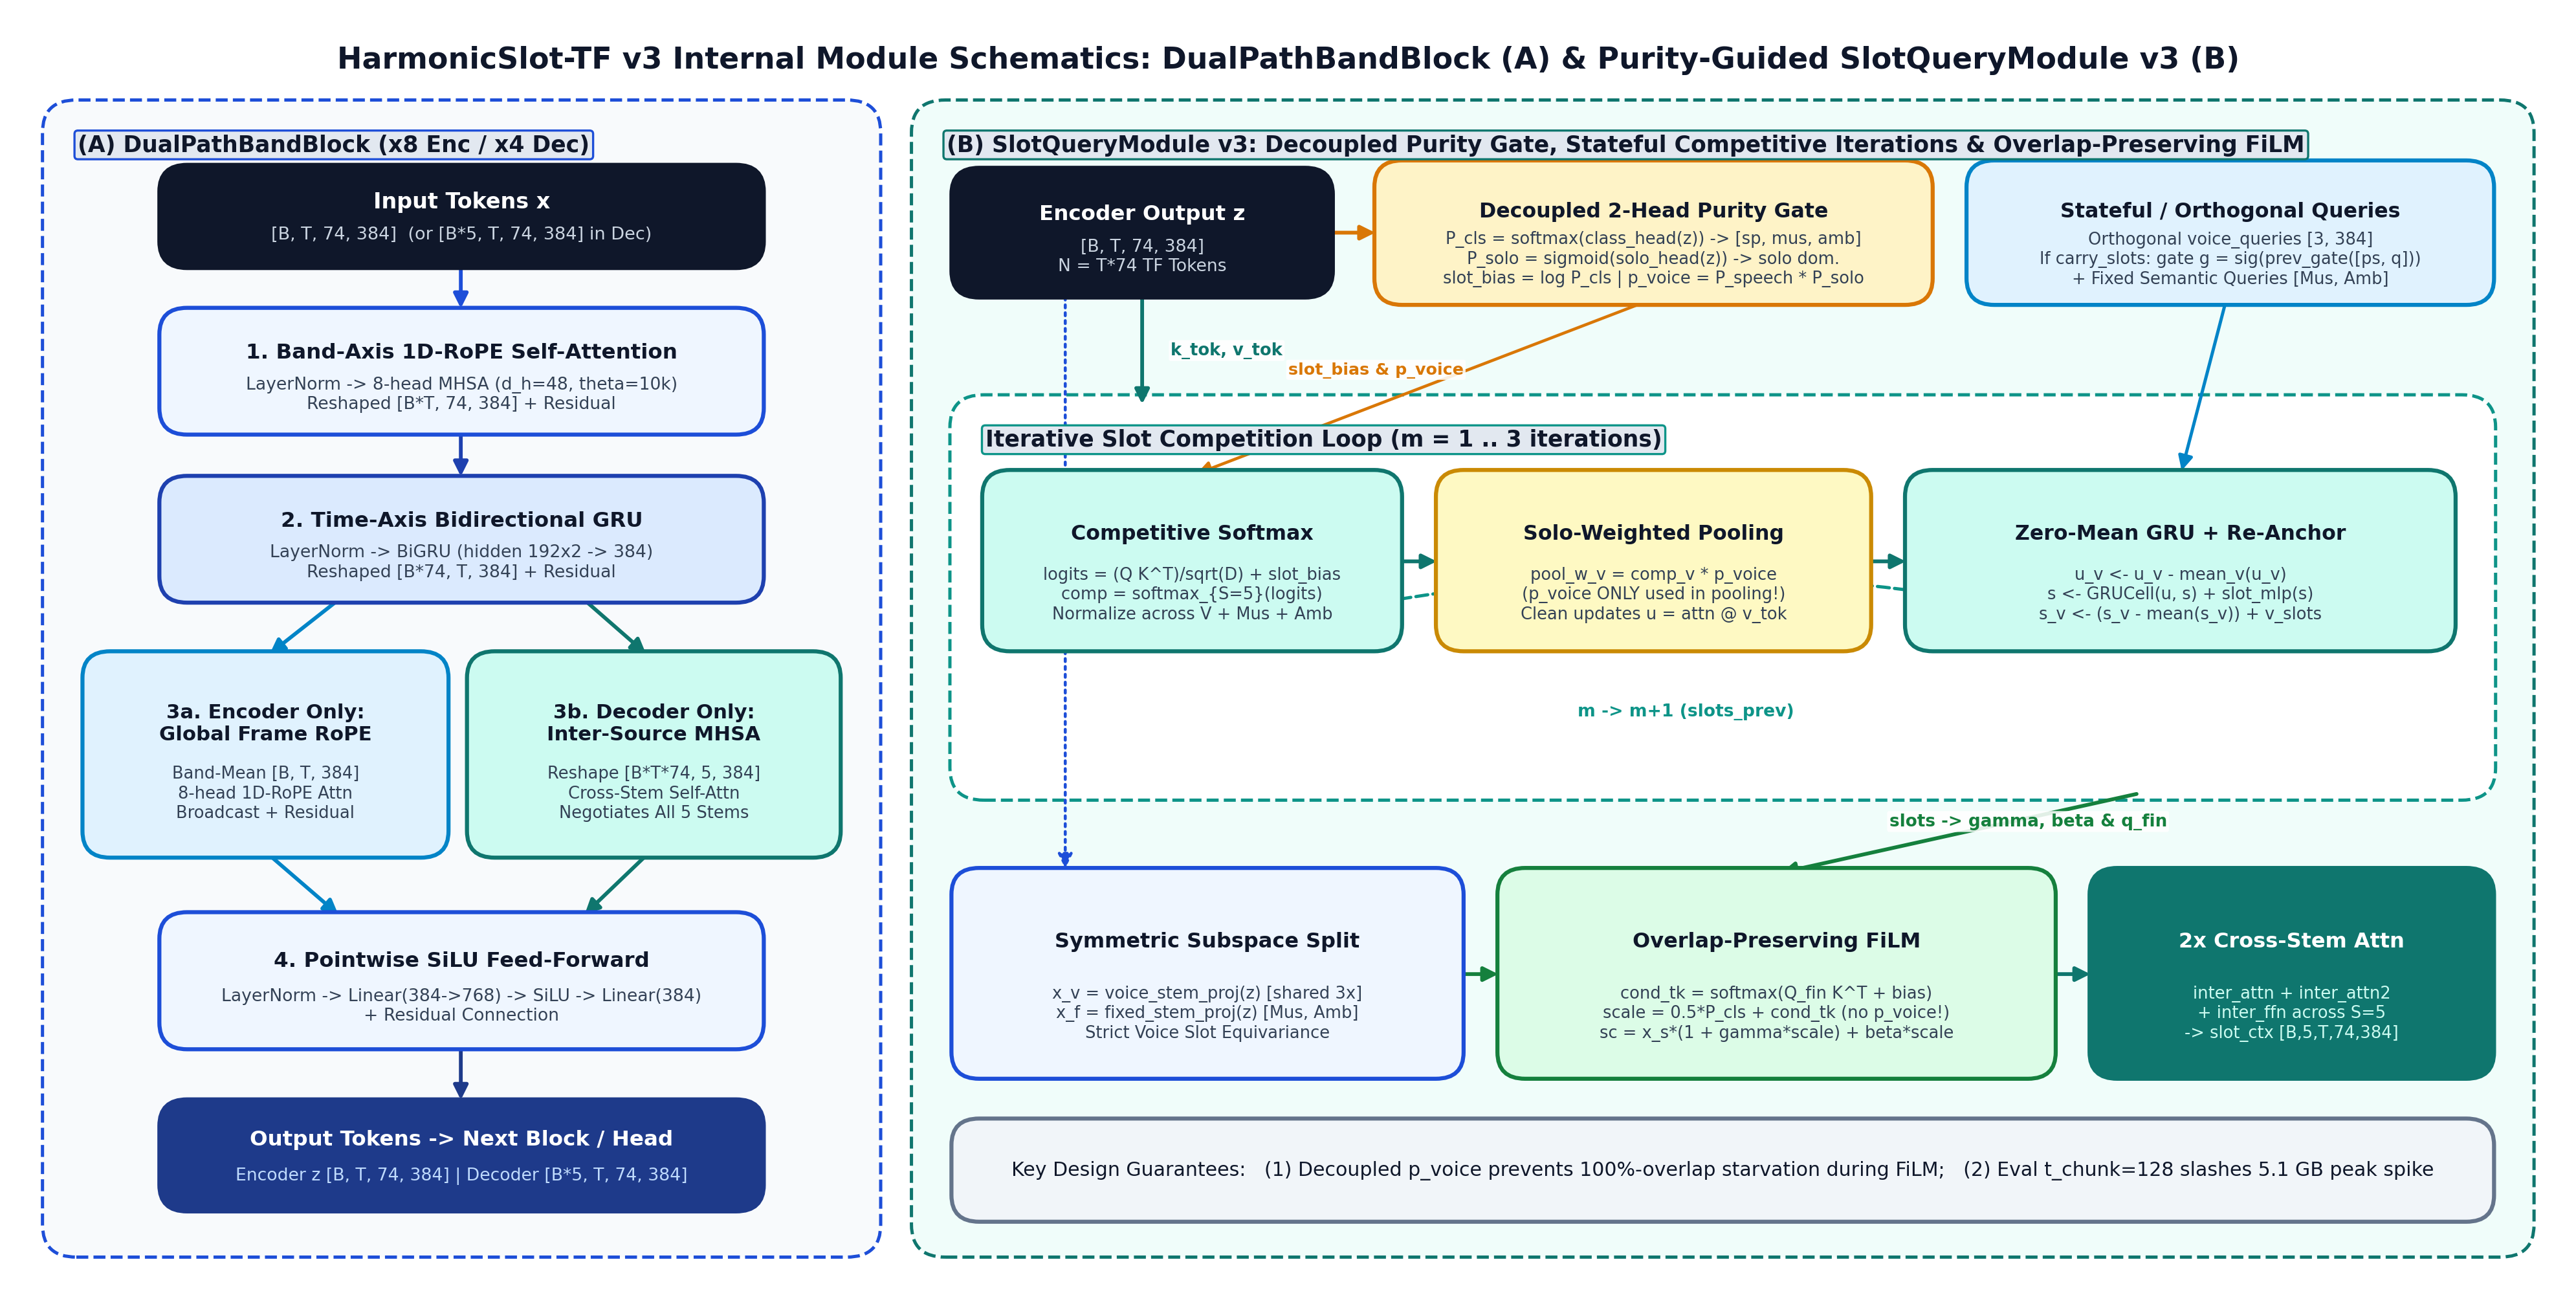
\includegraphics[width=\linewidth]{figures/fig_arch2_harmonicslot_block.png}
\caption{Internal module schematics: (A) \texttt{DualPathBandBlock} showing Band 1D-RoPE attention, Time BiGRU, Encoder global RoPE / Decoder per-$(t,k)$ inter-source attention, and SiLU FFN; (B) \texttt{SlotQueryModule v3} showing decoupled purity pooling ($P_{\text{solo}}$ isolated from FiLM) and symmetric subspace conditioning.}
\label{fig:arch2}
\end{figure}

\section{Hybrid Multi-Objective Loss \& Automated 48\,kHz Dataset Audit}
Stage~1 minimizes:
\begin{equation}
\mathcal{L}_{\text{total}} = \mathcal{L}_{\text{voice}} + \mathcal{L}_{\text{fixed}} + 1.0\,\mathcal{L}_{\text{xbleed}} + 0.1\,\mathcal{L}_{\text{mix\_cons}} + 0.3\,\mathcal{L}_{\text{act}} + 0.1\,(\mathcal{L}_{\text{cls}} + \mathcal{L}_{\text{solo}}) + 0.2\,\mathcal{L}_{\text{ortho}}.
\end{equation}
All training files passed an automated multi-model ML Purity Audit (Silero VAD + AudioSet AST + WavLM-Base-Plus-SV~\cite{chen2022wavlm}): (1) \textbf{Speech:} 2,378 clean 48\,kHz clips across 152 speakers in 5 languages (OpenSLR 83 UK English, 65 Tamil, 66 Telugu, 68 Mandarin, 103 Hindi; SNR $\ge 42$\,dB, floor $\le -58$\,dB, 9 mislabeled clips quarantined via WavLM-SV cosine outlier audit; disjoint 137 train / 15 unseen val speakers); (2) \textbf{Music:} 60 vocal-free MUSDB18-HQ~\cite{rafii2019musdb18hq} tracks (2 rejected by AST/Silero for hidden vocal bleed at $0.79/0.71$); (3) \textbf{Ambience:} 16 speech-free 48\,kHz DEMAND~\cite{thiemann2013demand} recordings across 8 rooms; and (4) \textbf{RIRs:} 400 OpenSLR 28 impulse responses ($360/40$), convolved onto $50\%$ of voice tracks alongside $50\%$ dual-mono ($L=R$) and $50\%$ 100\%-overlap mixtures.

\section{Stage-2 Full-Bin Cross-Stem De-Bleed Refiner (v2, 17.95\,MB)}
\texttt{CrossStemDebleedRefiner v2} ($8{,}973{,}540$ params, 17.95\,MB \texttt{bf16}: \texttt{voice\_net} $6{,}356{,}330$, \texttt{bg\_net} $2{,}599{,}450$, \texttt{voice\_wave\_net} $17{,}760$) operates directly at full 1,025-bin STFT resolution behind frozen Stage~1. For each target voice $v$, the remaining two voices are sorted by descending RMS ($Y_{o1} \ge Y_{o2}$) into a 35-channel feature tensor (log-compressed Re/Im of all 6 complex signals, per-reference log-magnitudes, 2-voice and 4-ref dominance ratios, and all 4 independent complex phase coherences). For Music ($+1.0$ stem flag) and Ambience ($-1.0$ flag), all three voices are sorted by descending RMS into a 36-channel tensor. Keeping full $5.33$\,ms resolution on top U-Net skips $h_0, h_1$ while using $\text{stride}=(2,2)$ on \texttt{down2}/\texttt{down3} ($21.3$\,ms bottleneck with $3/2$ Dual-Path BiGRUs) reduced A100-40GB 50-step training time by $3.48\times$ ($366.7\,\text{s} \to 105.4\,\text{s}$). The bounded complex cancellation filter and local-RMS ($5.3$\,ms) waveform polish follow:
\begin{align}
\hat{Y}_{\text{self}} &= \sigma(g_{\text{raw}} + 3.0)(1 + 0.50\,\Delta M_{\text{self}}) Y_{\text{self}} - 0.85\sum_{r=1}^{4} M_r Y_r + 0.35\,M_{\text{mix}} Y_{\text{mix}}, \\
\delta_{\text{wave}}(t) &= 0.15 \cdot \sqrt{\operatorname{AvgPool1d}_{k=257}(y^2)(t) + 10^{-12}} \cdot \tanh(\operatorname{Conv1d}([y, y_{\text{other}}, \text{bg}, \text{mix}])).
\end{align}
Wrapping \texttt{\_DualPathBottleneck} in \texttt{autocast(enabled=False)} (\texttt{fp32}) prevented PyTorch cuDNN \texttt{nn.GRU} from silently downcasting to \texttt{fp16} under \texttt{bf16} autocast (fixing $60/182$ zero-gradient tensors to $225/225$ non-zero gradients), while local-RMS gating reduced adversarial silent-pause leakage to $1.5\times 10^{-7}$ ($-136$\,dBFS). Figure~\ref{fig:arch3} depicts the complete Stage-2 U-Net and reference-sorting architecture.

\begin{figure}[h]
\centering
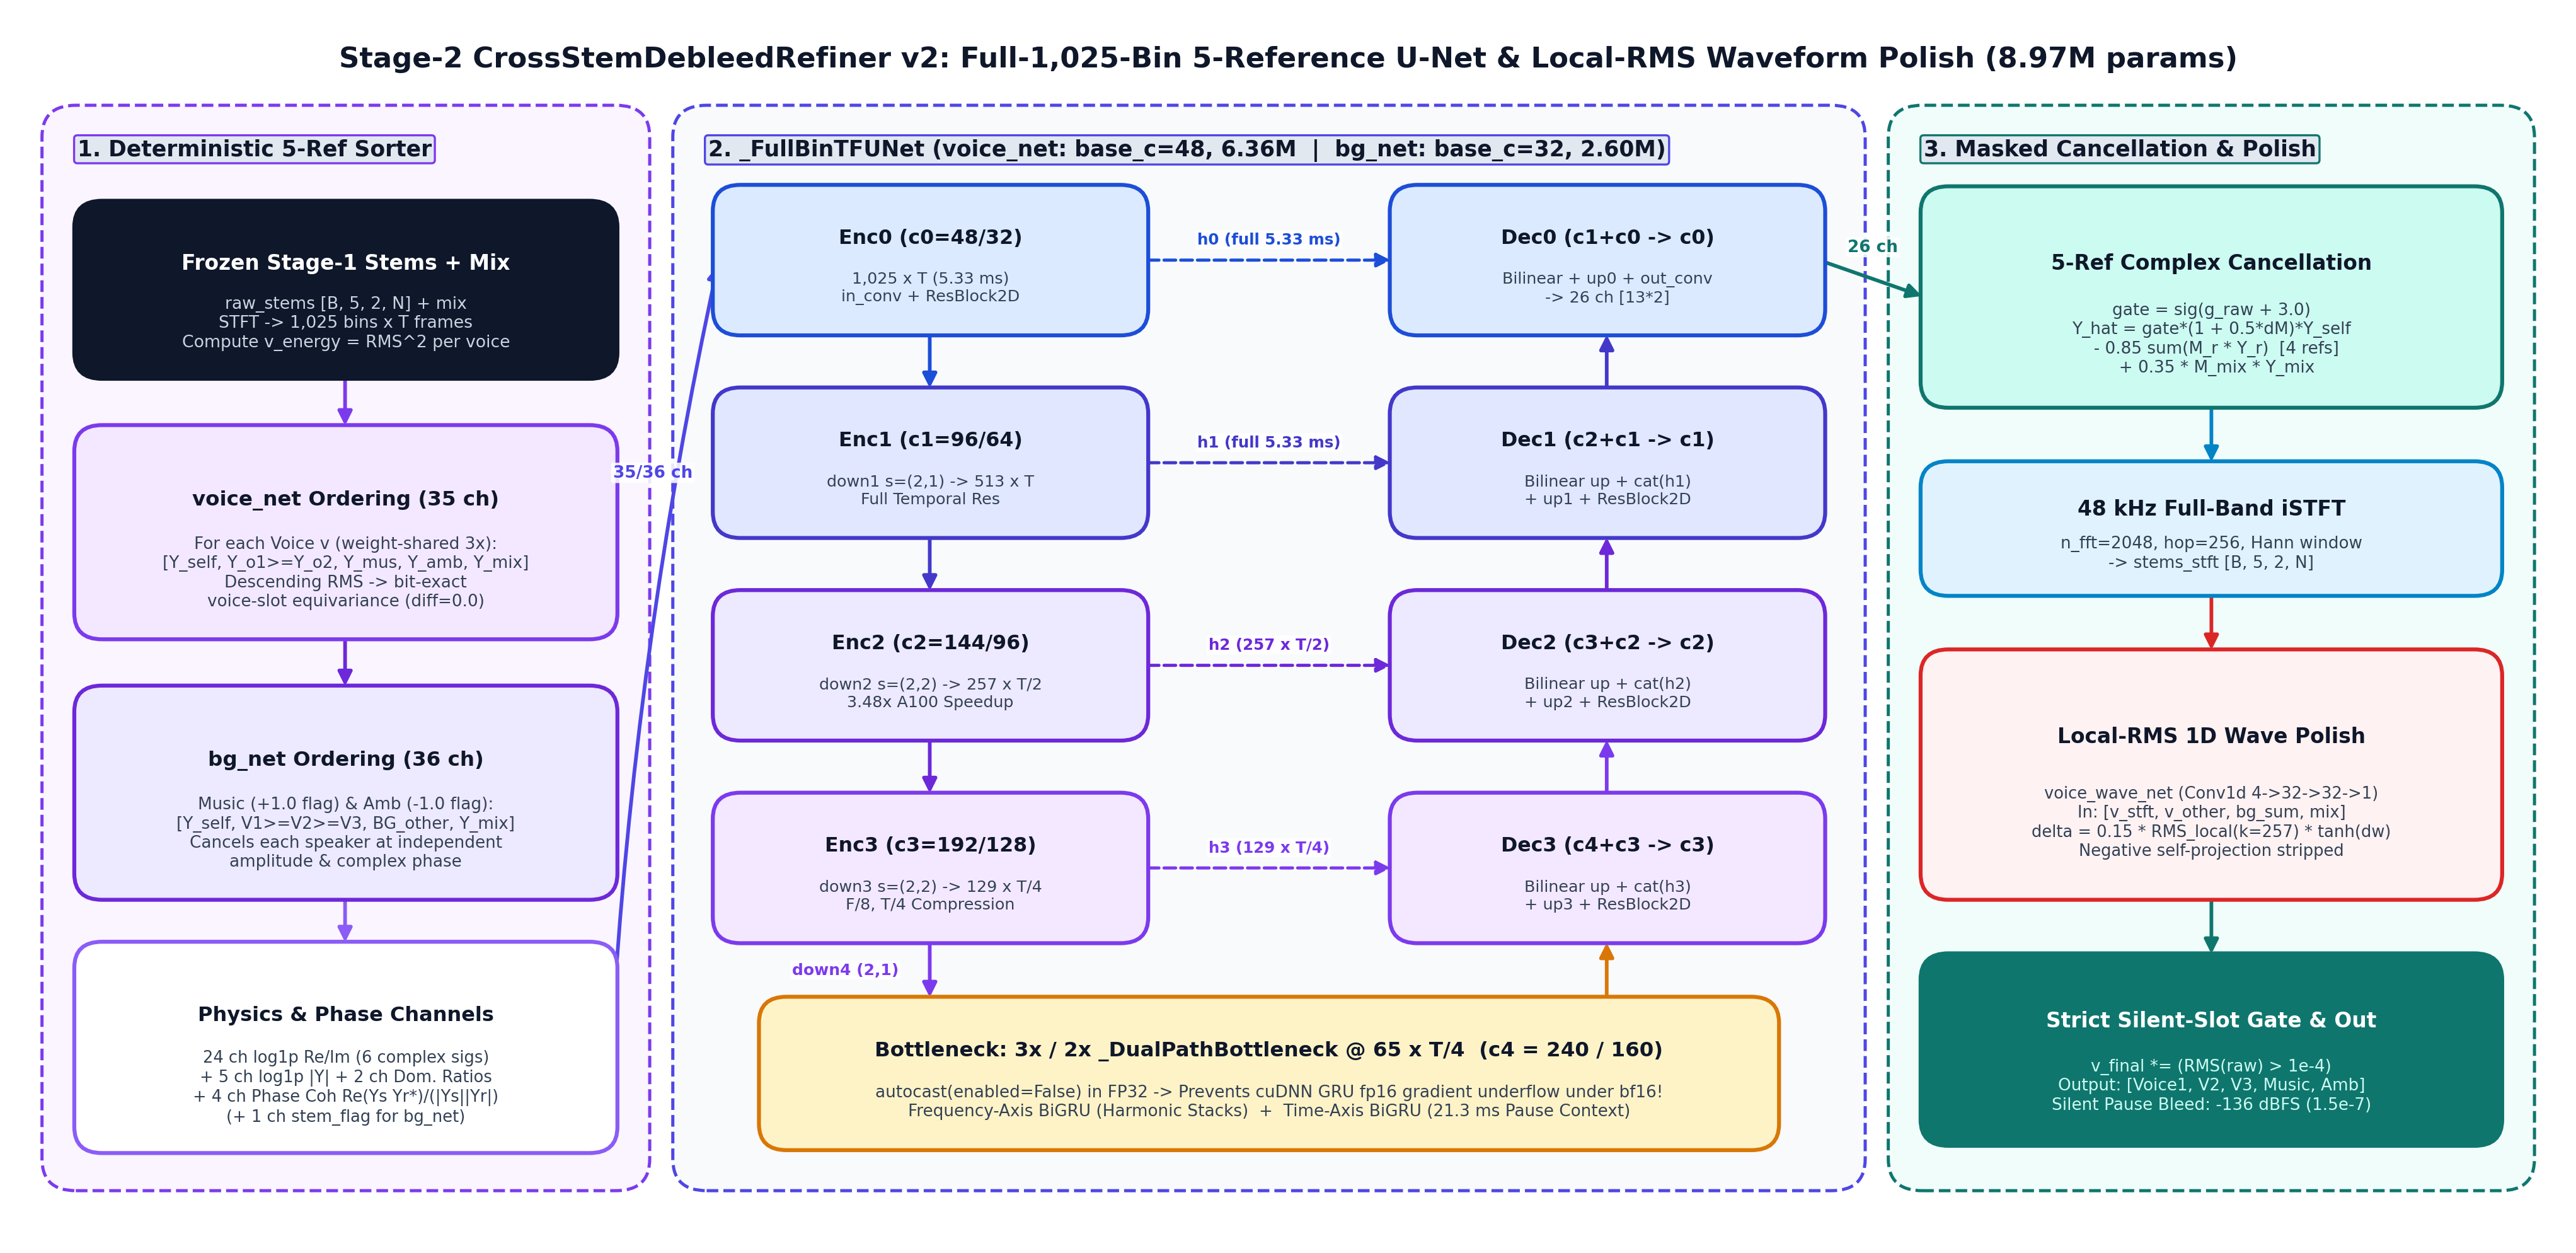
\includegraphics[width=\linewidth]{figures/fig_arch3_refiner_unet.png}
\caption{Architecture of \texttt{CrossStemDebleedRefiner v2} ($8.97$M params): deterministic descending-RMS 5-reference ordering, full-1,025-bin asymmetric-stride 2D U-Net with \texttt{fp32}-protected dual-axis bottleneck BiGRUs, 5-reference complex cancellation, and $5.3$\,ms local-RMS 1D waveform polish.}
\label{fig:arch3}
\end{figure}

\section{Consumer-GPU Inference Engineering (4.4$\times$ VRAM Reduction)}
Eliminating transient 5-stem materialization spikes via eval-only time-chunked slot conditioning ($t_{\text{chunk}}=128$), sequential per-stem decoder/enhancer loops, and immediate dead-tensor deallocation achieved verified FP32 numerical equivalence ($\max|\Delta|=8.05\times 10^{-7}$, mean $3.10\times 10^{-8}$) while cutting peak RTX~4060 Laptop 8\,GB VRAM by $76.6$--$77.2\%$ ($8.02 \to 1.88$\,GB at 6.0\,s; Figure~\ref{fig:vram}). Full chained Stage-1 + Stage-2 inference completes 6.0\,s 48\,kHz stereo chunks in $4.61$\,s ($1.30\times$ real-time).

\begin{figure}[h]
\centering
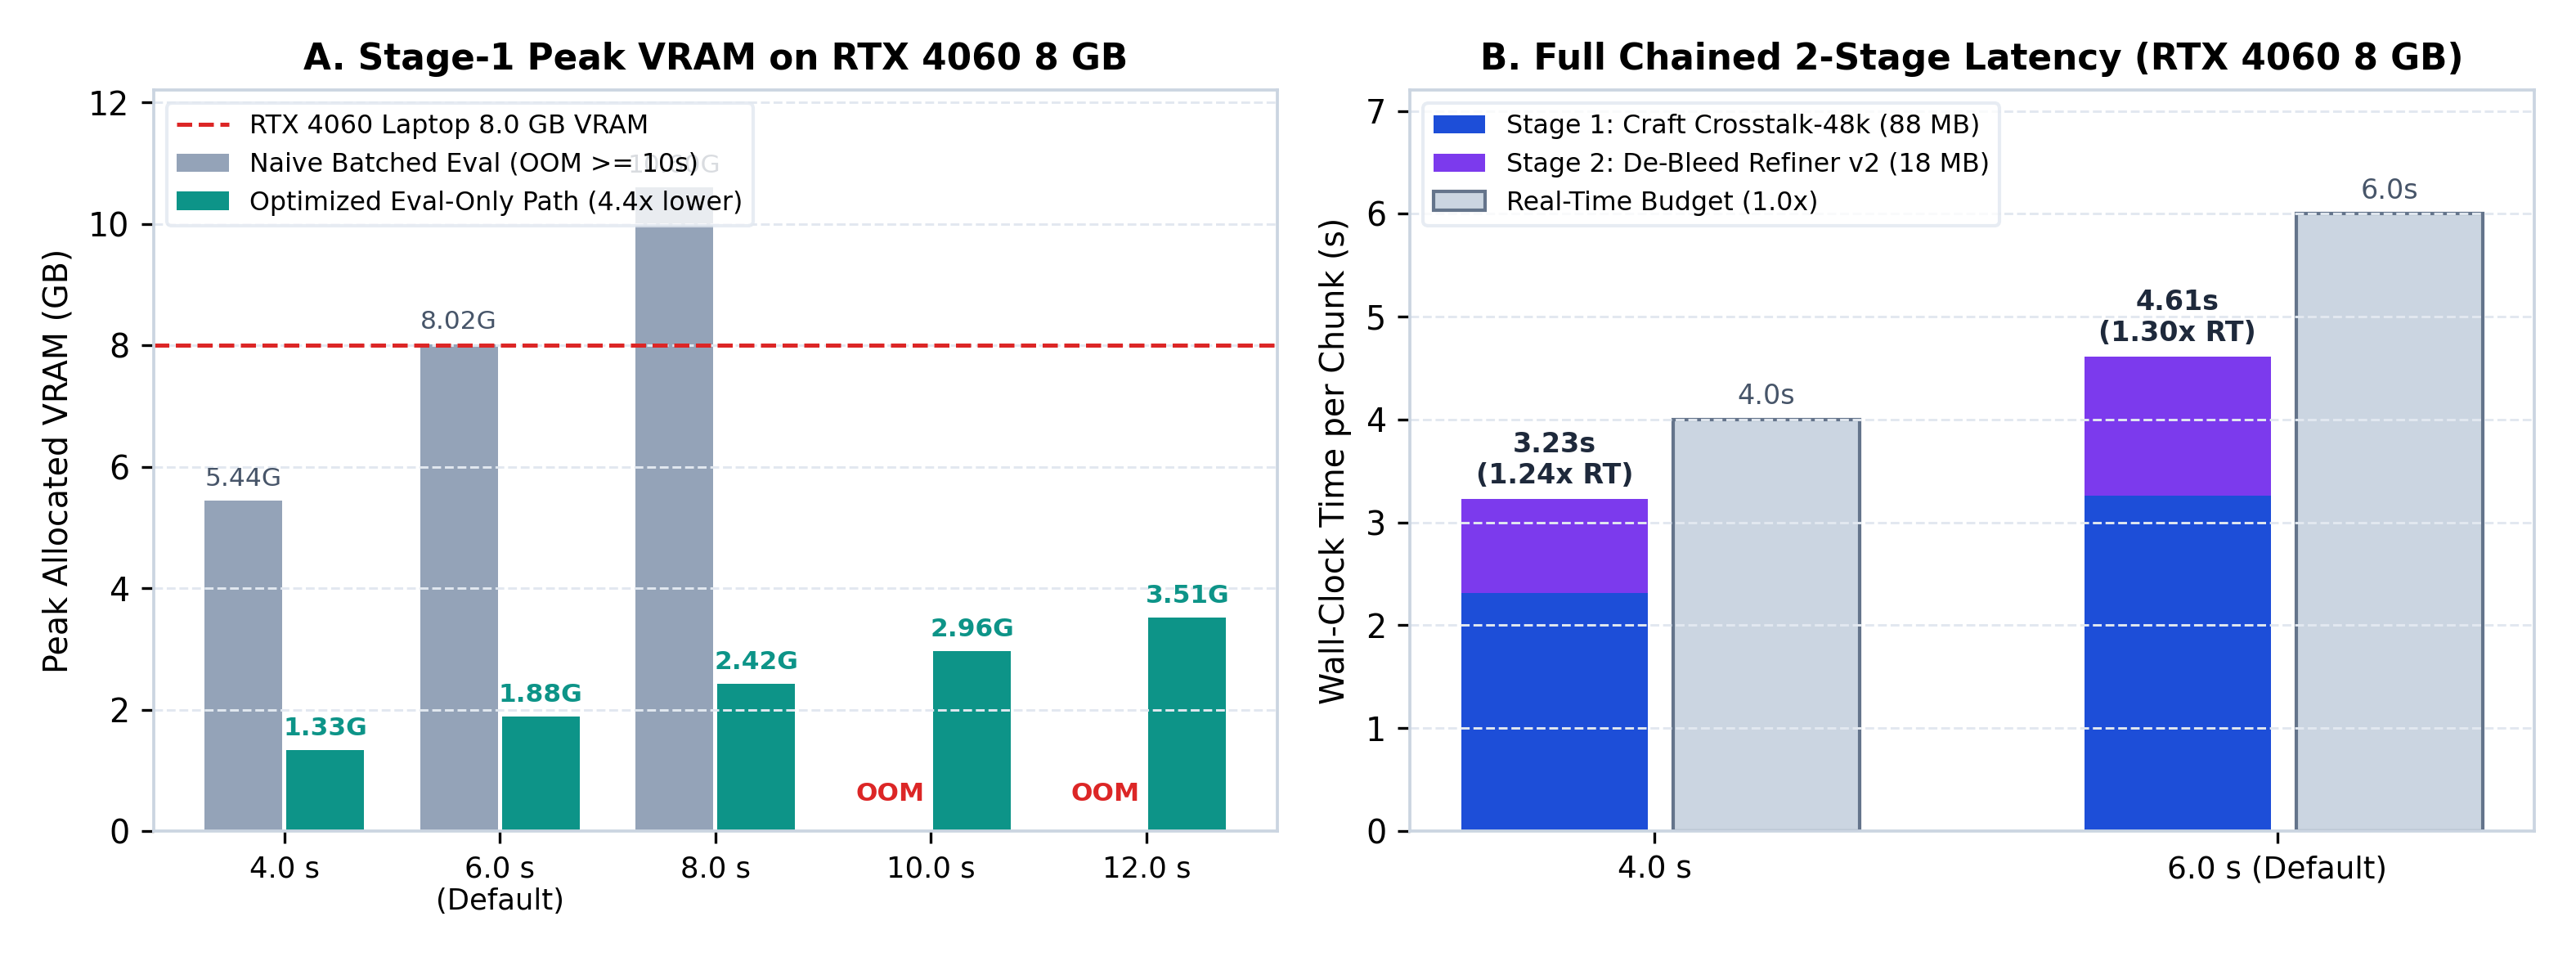
\includegraphics[width=\linewidth]{figures/fig4_vram_latency.png}
\caption{Measured NVIDIA GeForce RTX~4060 Laptop (8\,GB VRAM) \texttt{bf16} inference benchmarks.}
\label{fig:vram}
\end{figure}

\section{Complete Experimental Results \& Candid Failure Analysis}
\subsection{Phase-1 ($5\text{k}\to 17\text{k}$) and Phase-2 ($17.25\text{k}\to 21\text{k}$) Validation Trajectory}
Figure~\ref{fig:curves} and Table~\ref{tab:main_results} present the complete held-out EMA validation trajectory across all 23 logged checkpoints.

\begin{figure}[h]
\centering
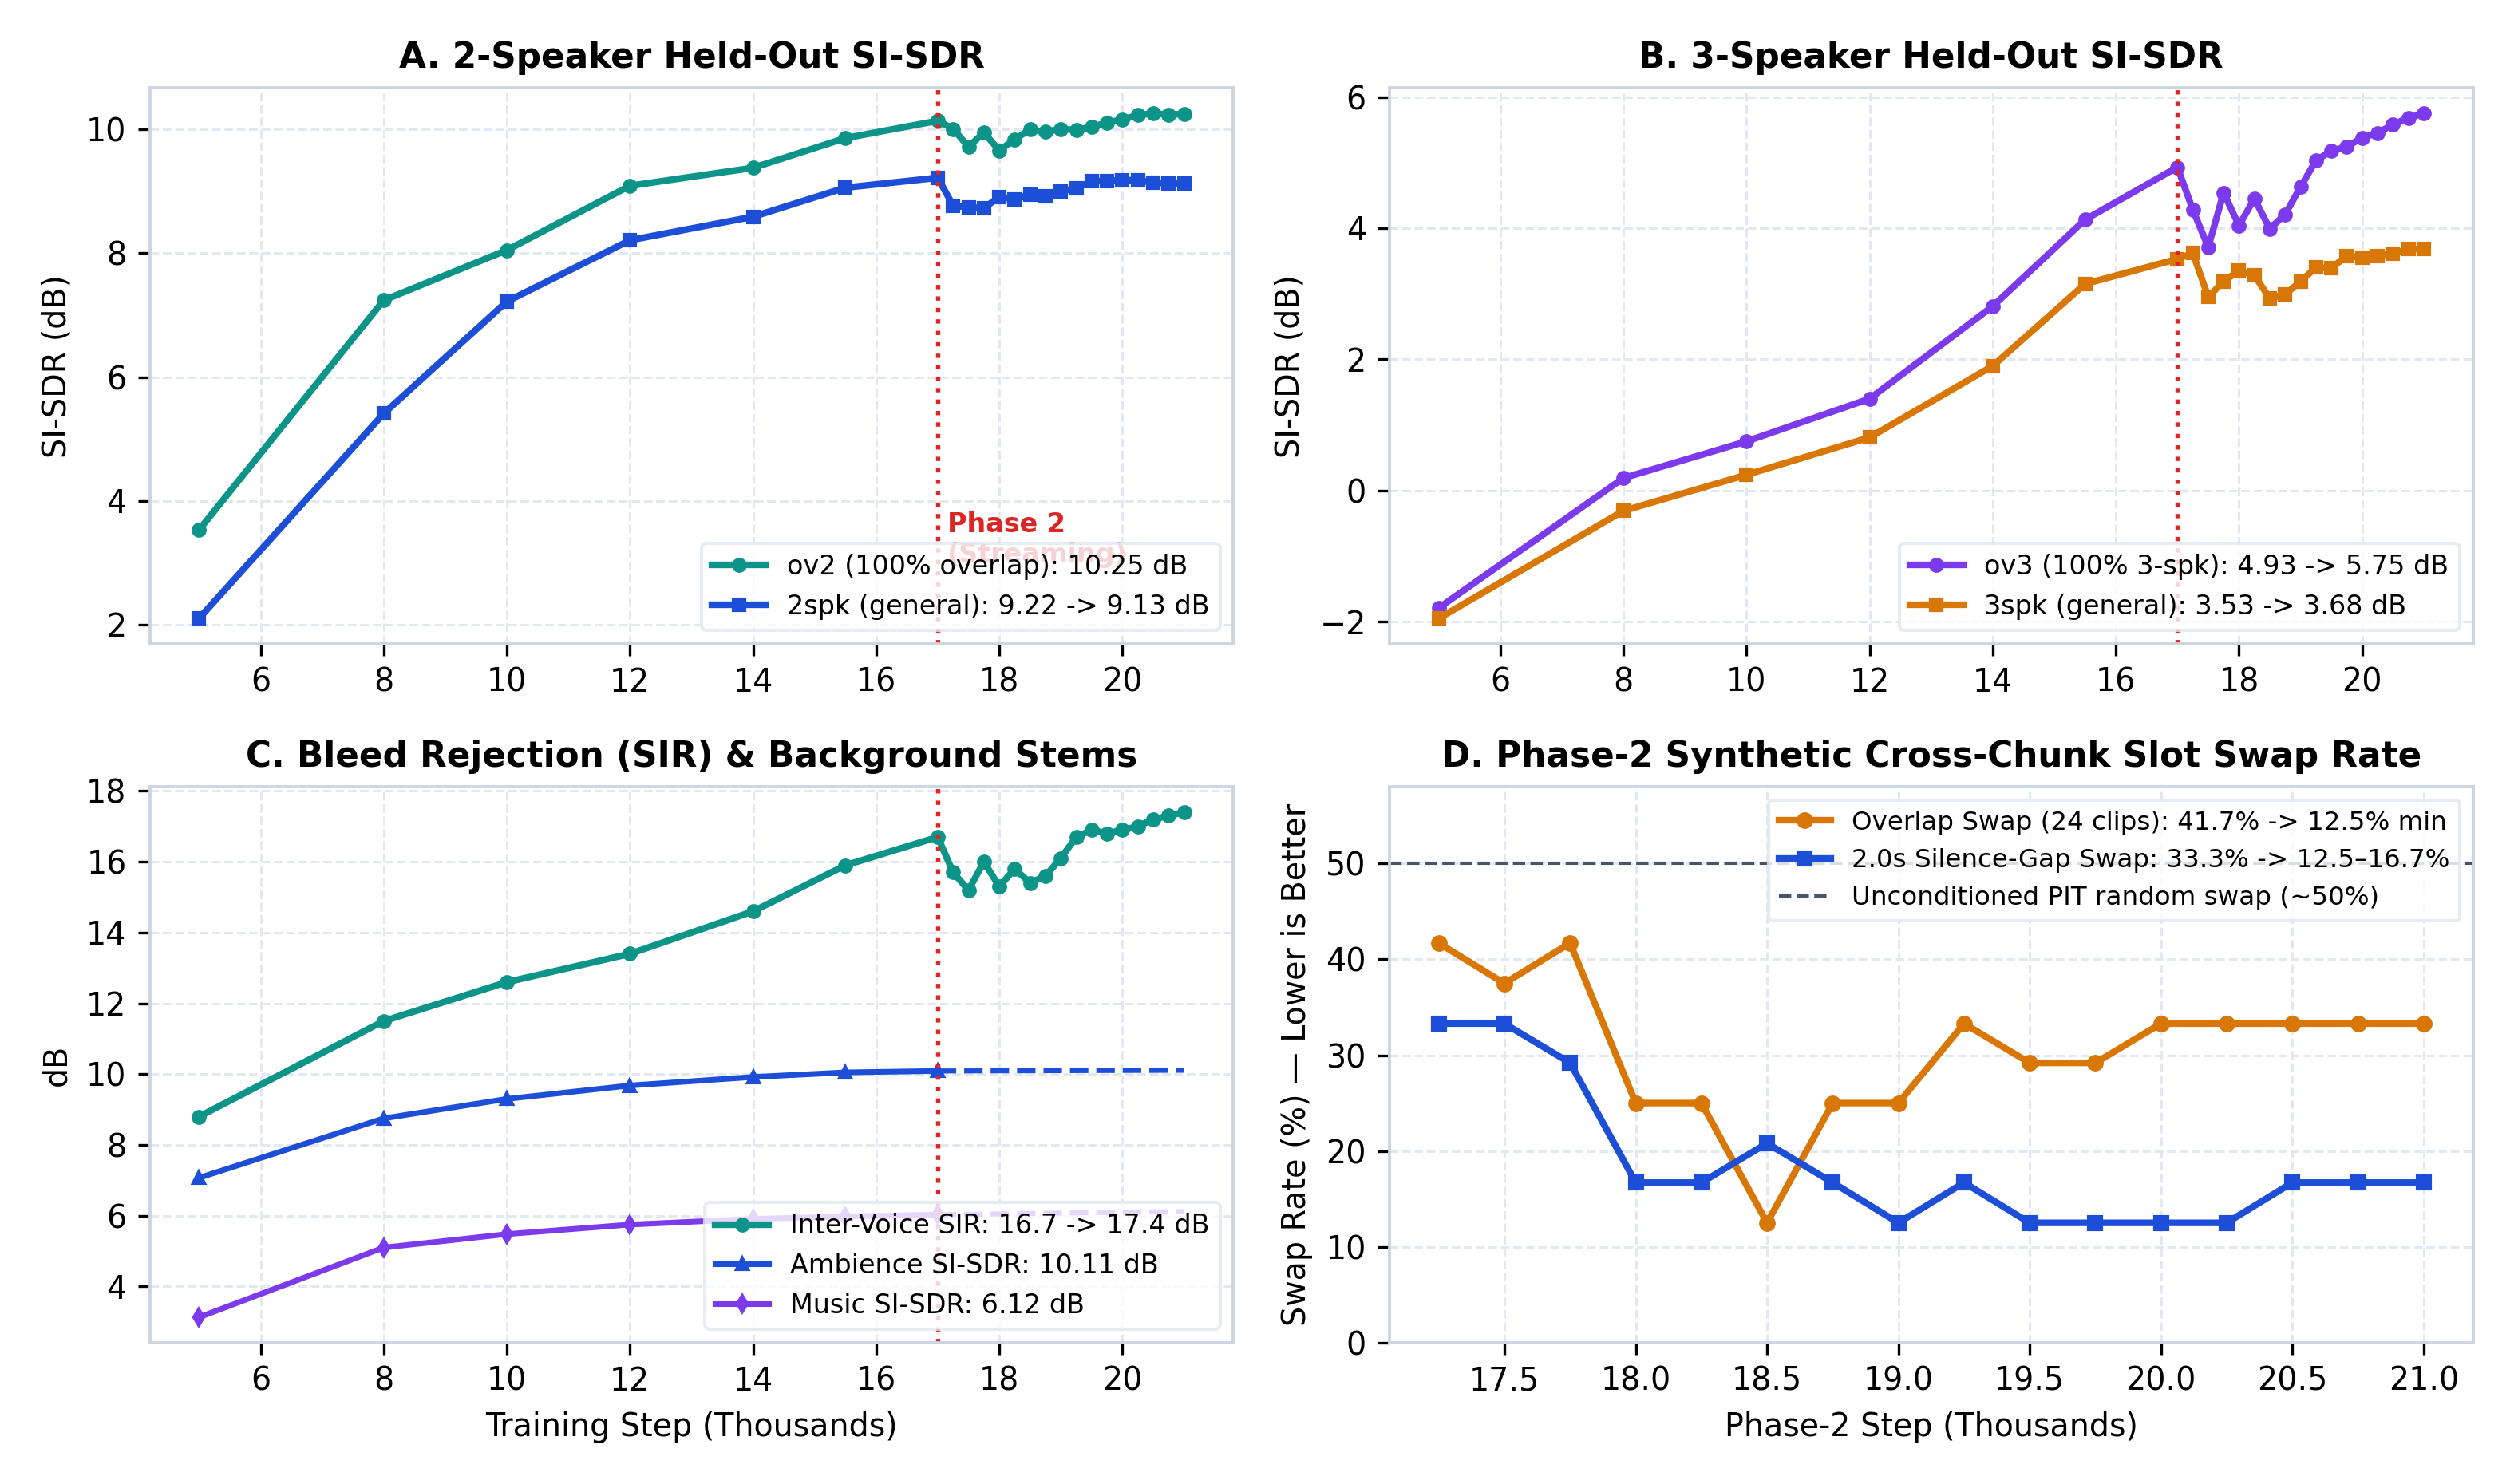
\includegraphics[width=\linewidth]{figures/fig1_training_curves.png}
\caption{Complete Phase-1 ($5\text{k} \to 17\text{k}$) and Phase-2 ($17.25\text{k} \to 21\text{k}$) EMA validation trajectories on held-out unseen speakers, music, ambience, and RIRs.}
\label{fig:curves}
\end{figure}

\begin{table}[h]
\centering
\caption{Complete logged EMA validation progression across Phase 1 and Phase 2 (15 unseen speakers, 50\% dual-mono).}
\label{tab:main_results}
\footnotesize
\begin{tabular}{lccccccccccc}
\toprule
\textbf{Phase / Step} & \textbf{2spk} & \textbf{ov2} & \textbf{3spk} & \textbf{ov3} & \textbf{SIR} & \textbf{Music} & \textbf{Amb} & \textbf{CntAcc} & \textbf{Swap} & \textbf{GapSwap} & \textbf{Unused} \\
\midrule
P1 --- 5,000 / 8,000 & 2.10 / 5.41 & 3.53 / 7.24 & $-1.95$ / $-0.31$ & $-1.79$ / 0.19 & 8.8 / 11.5 & 3.13 / 5.10 & 7.07 / 8.75 & 50.0 / 66.7\% & --- & --- & $-30.9$ / $-36.3$ \\
P1 --- 10,000 / 12,000 & 7.22 / 8.21 & 8.05 / 9.09 & 0.24 / 0.81 & 0.75 / 1.40 & 12.6 / 13.4 & 5.48 / 5.75 & 9.30 / 9.68 & 66.7 / 75.0\% & --- & --- & $-41.2$ / $-46.1$ \\
P1 --- 14,000 / 15,500 & 8.59 / 9.06 & 9.38 / 9.86 & 1.90 / 3.15 & 2.81 / 4.13 & 14.6 / 15.9 & 5.91 / 5.98 & 9.92 / 10.05 & 87.5 / 89.6\% & --- & --- & $-55.9$ / $-58.9$ \\
\textbf{P1 --- 17,000 (Best)} & \textbf{9.22} & 10.14 & 3.53 & 4.93 & 16.7 & 6.03 & 10.09 & \textbf{89.6\%} & 37.5\% & --- & $-58.9$ \\
\midrule
P2 --- 17,250 / 17,500 & 8.77 / 8.74 & 10.01 / 9.72 & 3.62 / 2.95 & 4.28 / 3.71 & 15.7 / 15.2 & 6.00 / 5.97 & 10.01 / 10.03 & 87.5\% & 41.7 / 37.5\% & 33.3\% & $-58.5$ \\
P2 --- 17,750 / 18,000 & 8.73 / 8.91 & 9.95 / 9.66 & 3.19 / 3.35 & 4.54 / 4.04 & 16.0 / 15.3 & 5.98 / 6.07 & 10.02 / 10.03 & 87.5\% & 41.7 / 25.0\% & 29.2 / 16.7\% & $-58.7$ \\
P2 --- 18,250 / 18,500 & 8.87 / 8.95 & 9.84 / 10.00 & 3.28 / 2.93 & 4.45 / 3.99 & 15.8 / 15.4 & 6.06 / 6.02 & 10.09 / \textbf{10.21} & 89.6\% & 25.0 / \textbf{12.5\%} & 16.7 / 20.8\% & $-58.8$ \\
P2 --- 18,750 / 19,000 & 8.92 / 9.00 & 9.96 / 10.01 & 2.99 / 3.19 & 4.21 / 4.63 & 15.6 / 16.1 & 6.03 / 6.02 & 10.07 / 10.09 & 87.5\% & 25.0\% & 16.7 / \textbf{12.5\%} & $-59.7$ / $-58.9$ \\
P2 --- 19,250 / 19,500 & 9.05 / 9.16 & 9.99 / 10.04 & 3.40 / 3.39 & 5.03 / 5.18 & 16.7 / 16.9 & 6.04 / 6.04 & 10.12 / 10.09 & 85.4\% & 33.3 / 29.2\% & 16.7 / \textbf{12.5\%} & \textbf{$-61.4$} \\
P2 --- 19,750 / 20,000 & 9.17 / 9.18 & 10.11 / 10.16 & 3.58 / 3.55 & 5.24 / 5.38 & 16.8 / 16.9 & 6.03 / 6.05 & 10.09 / 10.10 & 85.4\% & 29.2 / 33.3\% & \textbf{12.5\%} & $-59.0$ / $-57.9$ \\
P2 --- 20,250 / 20,500 & 9.18 / 9.14 & 10.23 / \textbf{10.26} & 3.58 / 3.61 & 5.45 / 5.58 & 17.0 / 17.2 & 6.07 / 6.08 & 10.11 / 10.07 & 87.5\% & 33.3\% & \textbf{12.5} / 16.7\% & $-58.9$ / $-60.7$ \\
\textbf{P2 --- 20,750 / 21,000} & 9.13 / 9.13 & 10.24 / 10.25 & \textbf{3.68 / 3.68} & 5.68 / \textbf{5.75} & 17.3 / \textbf{17.4} & 6.11 / \textbf{6.12} & 10.10 / \textbf{10.11} & 87.5\% & 33.3\% & 16.7\% & $-61.2$ / $-59.6$ \\
\bottomrule
\end{tabular}
\end{table}

\subsection{Negative Finding \#1: Phase-2 Out-of-Domain Collapse on Real YouTube Audio}
Despite Phase~2's synthetic gains, real-world 128\,kbps YouTube shouting clips (\emph{Kitchen Nightmares} and \emph{Delhi Metro Fight}) exposed severe single-slot collapse ($V_2$ suppressed to $-58.3 / -49.7$\,dBFS while $V_3$ absorbed both speakers; Figure~\ref{fig:ood}). Turning off \texttt{carry\_slots} (\texttt{stream=OFF}) rescued \emph{Kitchen Nightmares} ($V_2: -58.3 \to -33.6$\,dBFS), proving an asymmetric hot/cold carried-slot starvation effect when Chunk~1 activates only one slot above $0.65$; yet Phase~2 still collapsed noisy \emph{Delhi Metro} ($-49.3$\,dBFS) due to its solo/gap-chunk training prior under lossy MP3 compression. By contrast, \textbf{Phase~1 cleanly separated both real clips}, and chaining Refiner~v2 behind Phase~1 reduced quiet-frame bleed floors by $-14.1$ to $-21.9$\,dB and cut $V_2$--$V_3$ envelope correlation by $56\%$ ($0.303 \to 0.132$).

\begin{figure}[h]
\centering
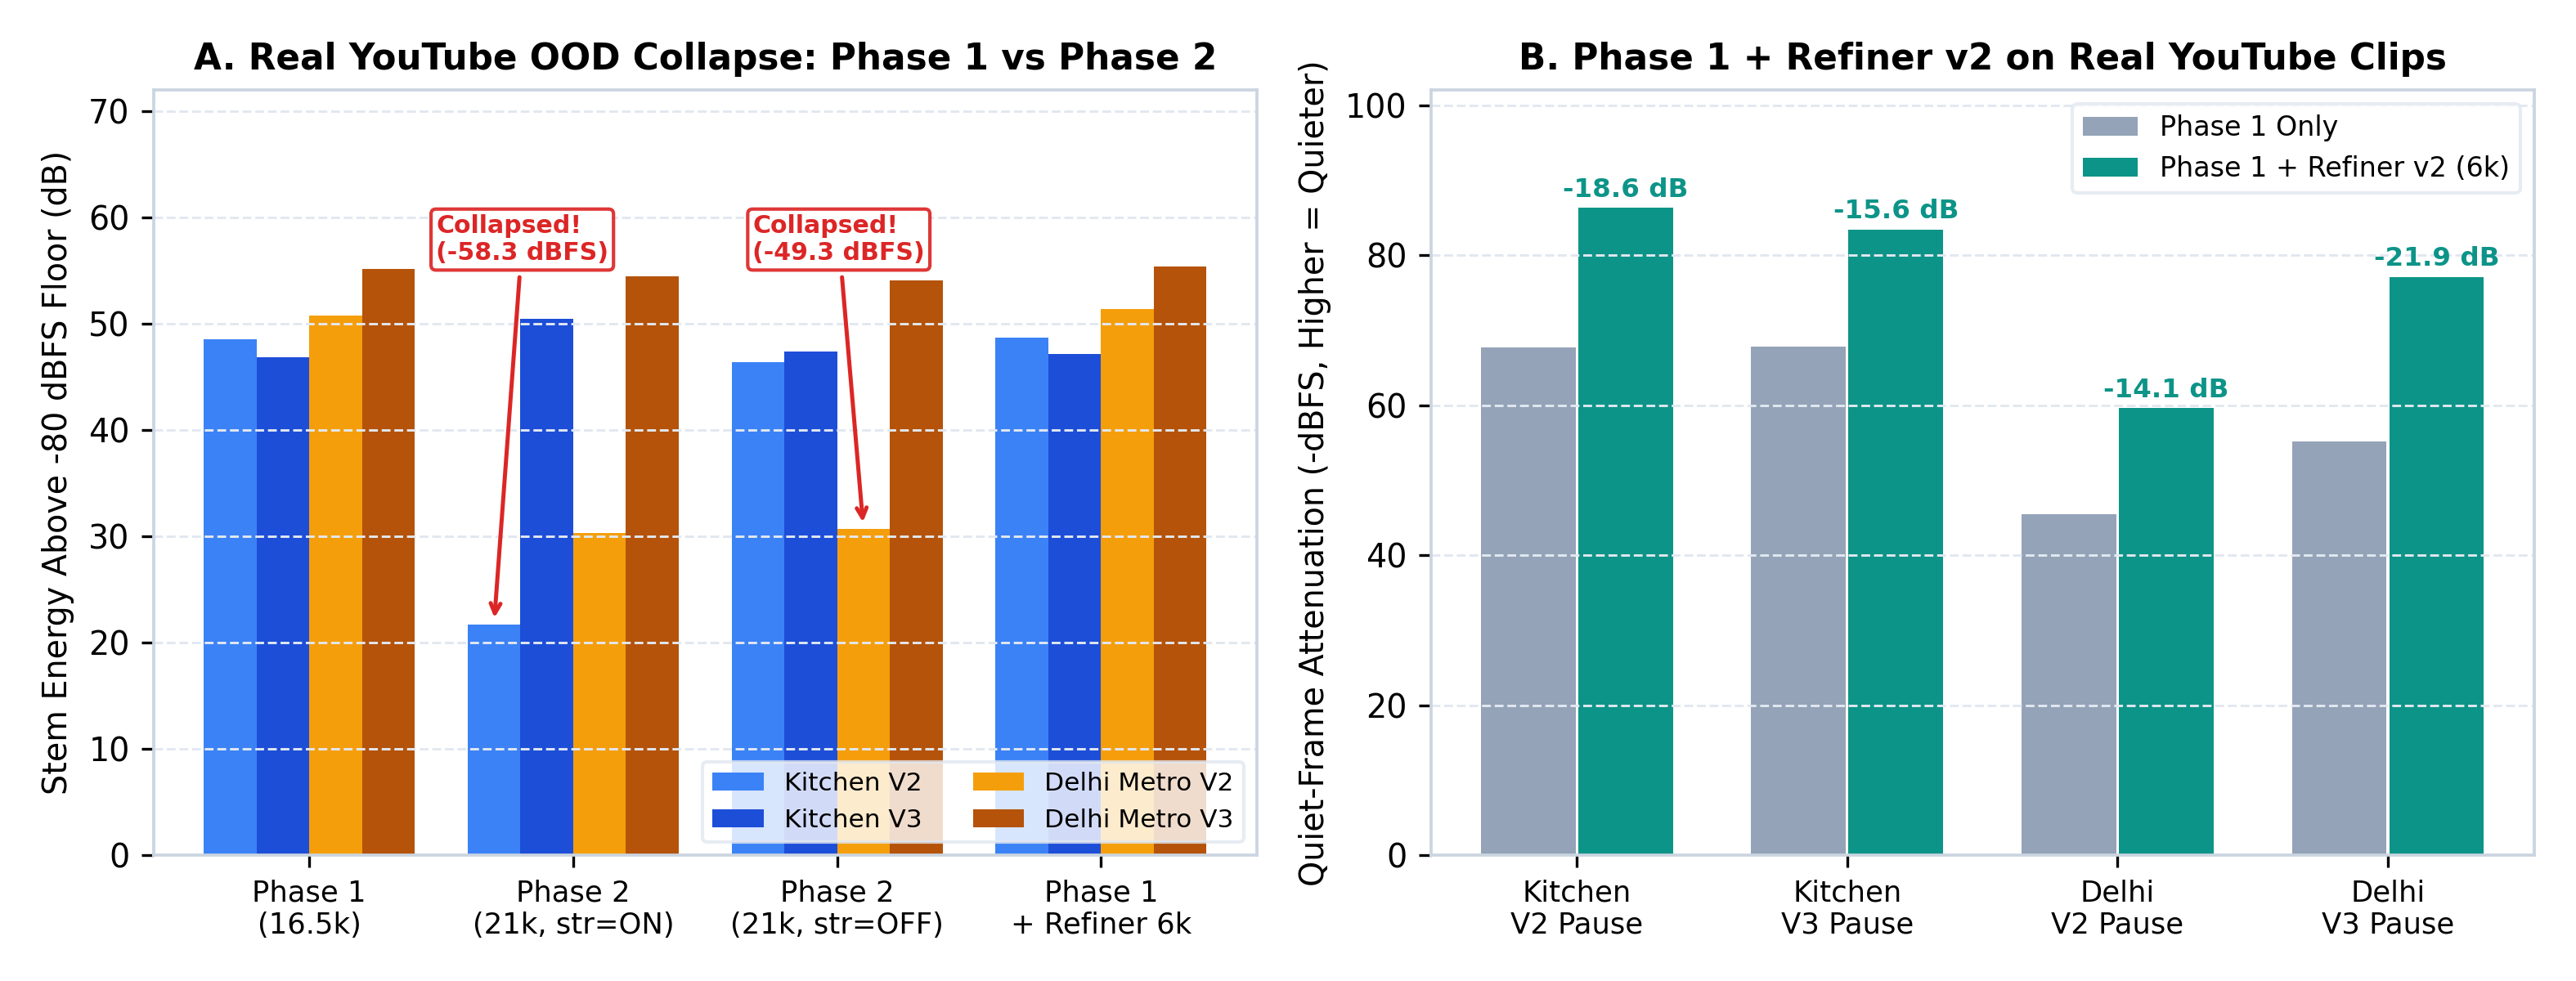
\includegraphics[width=\linewidth]{figures/fig2_domain_collapse_ab.png}
\caption{Real-world 128\,kbps YouTube OOD collapse diagnostic (left) and Phase 1 + Refiner v2 cleanup (right).}
\label{fig:ood}
\end{figure}

\subsection{Negative Finding \#2: Conv U-Net Refiner Excels on Pauses/Background, Plateaus on Active Overlap}
As shown in Figure~\ref{fig:refiner}, chaining \texttt{CrossStemDebleedRefiner v2} (step 6,000) behind an unseen Stage-1 checkpoint (step 20,250) on unseen speakers yields $-19.1$\,dB pause ghost bleed ($+5.97$\,dB pause-clip SI-SDR), $-44.3$\,dB quieter empty slots on solo speakers ($+0.10$\,dB solo SI-SDR), and $35$--$42\%$ lower vocal bleed inside Music and Ambience. However, on 100\% simultaneous active overlap, SIR improved by only $+2.2$\,dB (2-speaker) and $+2.4$\,dB (3-speaker) because a 2D Conv U-Net downsampled $16\times$ in frequency cannot untangle interleaved harmonic combs across all 1,025 bins simultaneously, and silent-frame loss ($\lambda_{\text{bleed}}=3.0$) favors pause gating.

\begin{figure}[h]
\centering
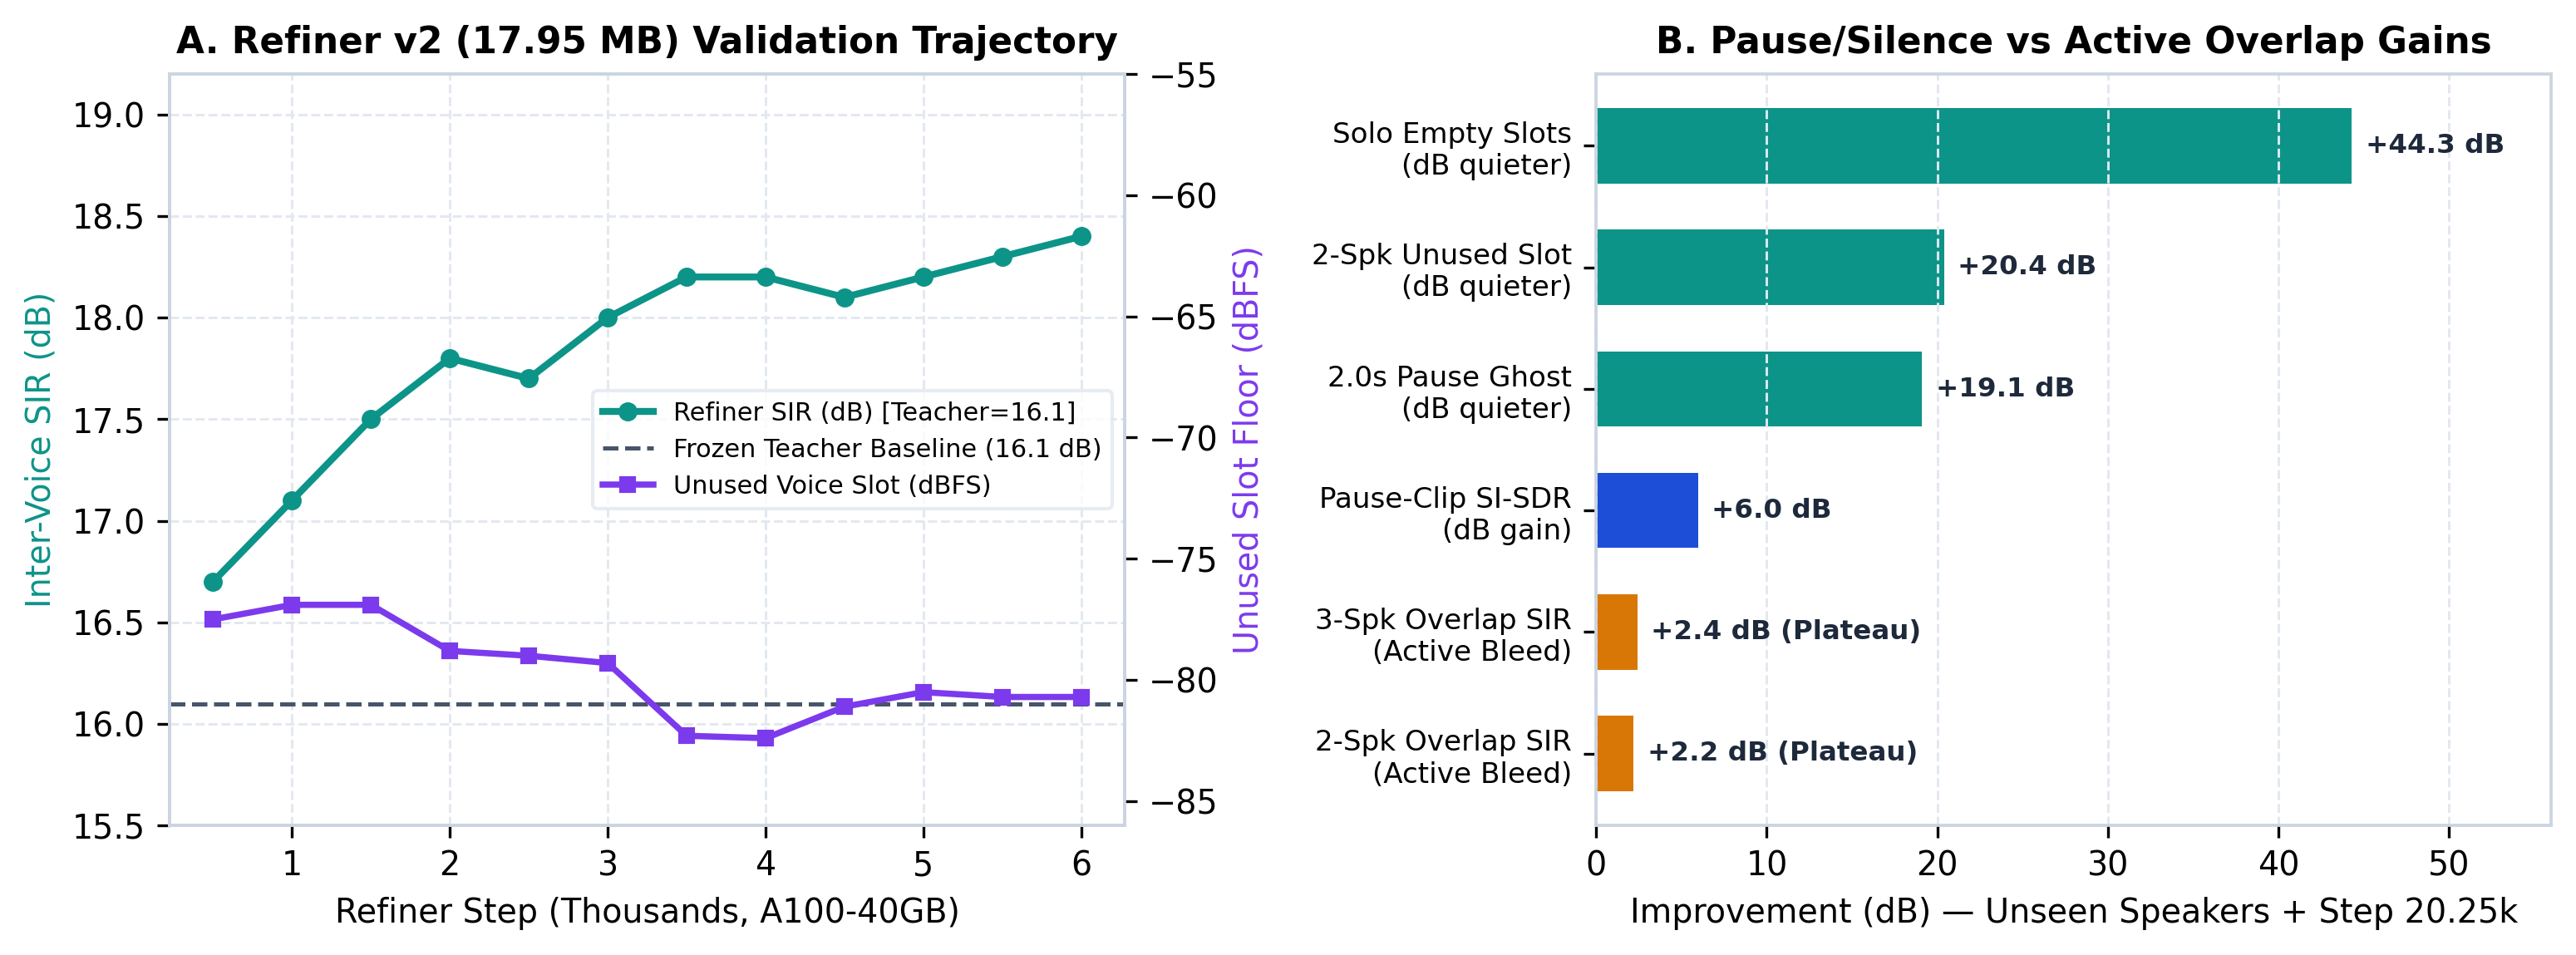
\includegraphics[width=\linewidth]{figures/fig3_refiner_ab.png}
\caption{Refiner v2 validation trajectory across 6,000 A100-40GB steps (left) and honest pause vs.\ active-overlap breakdown (right).}
\label{fig:refiner}
\end{figure}

\section{Open-Source Release \& Community-Funded v4 Roadmap}
All code, four ComfyUI nodes (\texttt{ComfyUI-HarmonicSlotTF}), pre-wired workflows, and all three \texttt{bf16} checkpoints (\texttt{phase1\_step17000} [SHA-256 \texttt{d75bfb4d...}], \texttt{phase2\_step21000} [\texttt{a0f655c8...}], and \texttt{refiner\_v2\_step6000} [\texttt{af203b3b...}]) are released openly at \url{https://github.com/SachiPoonga/Craft-Crosstalk-48k} (MIT for code/nodes; CC BY-NC-SA 4.0 for research weights). Community sponsorships via Ko-fi (\url{https://ko-fi.com/sachipoonga}) and PayPal directly fund \textbf{Craft Crosstalk-48k v4}: (1) scaling from 137 to $1{,}000+$ diverse CC0/CC-BY speakers with shouting and MP3/AAC codec augmentation; (2) full-resolution $>4.6$\,kHz bands + TF-GridNet-style full-bin cross-frequency harmonic attention trained specifically on simultaneous overlap; and (3) external frozen neural speaker verification (\texttt{WavLM-SV}) inside ComfyUI OLA for zero-collapse long-audio tracking.

\bibliographystyle{plain}
\bibliography{references}
\end{document}
